\section{Priority Scheduling}
\subsection{Data Structures}
\paragraph{A1: (5 marks)}
Copy here the declaration of each new or changed `struct' or `struct' member, global or static variable, `typedef', or enumeration.  Identify the purpose of each in 25 words or less.

synch.h:\\
Added to struct lock :
\begin{verbatim}
    int priority;               /* Caches priority of threaads in lock. */
    struct list_elem elem;      /* Used in thread.c */
\end{verbatim}
Locks now cache the priority of the most important thread in their waiting list (this number is PRI\_MIN for empty waiting lists).\\ \\

thread.h:
\begin{verbatim}
/* Lists various structures that thread can be waiting on. */
enum blocker_type
  {
    NONE,      /* Thread is running or in ready list. */
    SEMA,      /* Thread is waiting on a semaphore. */
    LOCK,      /* Thread is waiting on a lock. */
    COND       /* Thread is waiting on a conditional. */
  };
\end{verbatim}

Added to struct thread:
\begin{verbatim}
    /* Added for priority sorting and donations. */
    struct list locks;                  /* Locks acquired by the thread. */
    void *blocker;                      /* Struct that blocks this thread.*/
    enum blocker_type type;             /* What is blocking the thread? */
\end{verbatim}
Threads now keep track of the locks they have acquired and the structure (if any) that they are waiting on.


\subsection{Algorithms}
\paragraph{A2: (10 marks)}
Explain the data structure used to track priority donation. Give a diagram that illustrates a nested donation in your structure.
\\
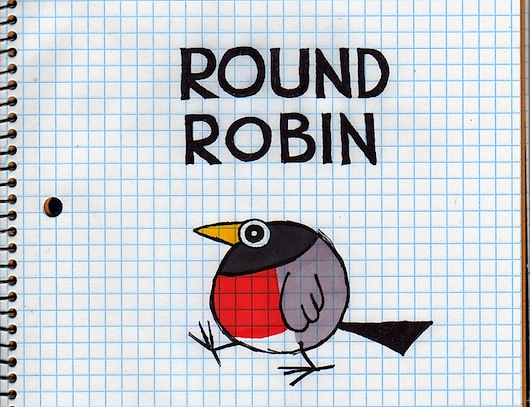
\includegraphics{roundrobin1}

Our implementation of priority donation does not rely on a single data structure. Instead, it is divided between struct lock and struct thread. Threads keep track of the locks they acquire, as well as the type of and pointer to the synch struct that they are waiting on, if applicable. Locks cache the priority of their most important waiting thread, avoiding unnecessary (and possibly recursive) calls into that thread to find out its priority.

In addition, the waiting lists for semaphores (by extension, locks) and condition variables order threads by priority, which makes it possible to track priority passively: finding the highest priority in a list of threads is simply a matter of looking at the head.

When a thread attempts to acquire a lock that is held by another thread, the lock checks if its priority is higher than the cached priority. If it is, the newly blocked thread\'s priority is \"donated\" to the holder thread. This is done by reinserting the lock into the holder thread's list of acquired locks, ordered by decending donated priority. Again, since these locks are listed in order, finding the lock donating the highest priority is a simple matter of looking at the head of this list (and the thead's effective priority can be easily calculated by comparing this with its base priority).

If priority donation updates a blocked thread's priority, we may need to recursively propogate this new donated priority if the blocker is a lock. Firstly, the blocked thread notifies the structure it is waiting on to re-order its waiting list to reflect the change of priority.
In the case of a semaphore, the blocked thread whose priority was modified is simply reinserted into the list (condition variables reinsert the semaphore that blocks the thread in question).
In the case of a lock, the waiting list is reordered like it is for semaphores, and if the lock determines that the highest priority has changed, it notifies the thread that holds it to reorder its list of acquired locks. If this thread is also blocked, the recursion continues.

\paragraph{A3: (5 marks)}
How do you ensure that the highest priority thread waiting for a lock, semaphore, or condition variable wakes up first?

Our implementation guarantees that the lists of waiting threads inside semaphores (by extension, locks) and condition variables are sorted in order of decreasing effective priority.

We maintain this guarantee by inserting threads into the waiting list with list\_insert\_ordered(), which uses an auxiliary function to compare thread priorities.
When a thread's effective priority changes through priority donation, if this thread is waiting in a list, we reinsert the thread into the list, thus maintaining its order. If it waiting on a lock, if the highest priority of the lock's waiting list is changed, this change is propagated to the holder of the lock.

When a semaphore, lock or condition variable wakes up a thread, it simply pops the front of the waiting queue, which we know is ordered. Hence when a thread is released from the waiters list, it is guaranteed to be (one of) the thread(s) with highest priority.

\paragraph{A4: (5 marks)}
Describe the sequence of events when a call to lock\_acquire() causes a priority donation.  How is nested donation handled?

  Firstly, thread A acquires lock 1.
    this sets the lock's holder to A and adds the lock into thread A\'s list of acquired locks.

  Then, thread B calls lock\_acquire() on lock 1
  Lock 1 has already been acquired, so
    update what thread B is blocking on (record the type of blocker and a pointer to it)
    check whether priority donation is needed (in this case it is)
      this updates the lock's cached priority, which is used by 
    now we take the lock's holding thread (i.e. thread A) and reorder its list of locks to place the lock donating the highest priority at the head. This thus indirectly causes thread B to donate its priority to thread A, assuming the highest donated priority thread A is receiving is from lock 1.
    \#\#\# TODO: make sure thread\_get\_priiority is explained in A2.

    Then, we check if we need to recurse. TODO: finish this part

\paragraph{A5: (5 marks)}
Describe the sequence of events when lock\_release() is called on a lock that a higher-priority thread is waiting for.

We shall assume that the higher priority priority thread (say thread B) is at the head of the lock\'s waiters list, and is donating its priority to the thread holding the lock (say thread A).

Firstly, thread A calls lock\_release(). This resets the lock's holder to NULL and removes the lock from thread A\'s list of acquired locks (interrupts are also disabled here to synchronise access to this list as it may be accessed in an interrupt handler).

The lock's cached priority is then recalculated (by getting the priority of the 2nd waiting thread, or returning PRI\_MIN if it doesn't exist) before sema\_up() removes the 1st waiting thread (say thread B) from the waiters list and calls thread\_unblock() on it.

This function resets thread B\'s blocker pointer and enum, sets its status to THREAD\_READY and inserts it into the ready list.

In this case, thread B\'s effective priority is now higher than the currently running thread A (as removing the lock from thread A\'s list of locks also removes any priority which it donated), so it gets must get placed at the head of the ready\_list (since thread A previously held the highest priority in ready\_list before it lost its donated priority and awakened thread B). A call to thread\_yield() is also triggered, causing thread B to pre-empt thread A and begin running.

\subsection{Synchronisation}
\paragraph{A6: (5 marks)}
Describe a potential race in thread\_set\_priority() and explain how your implementation avoids it.  Can you use a lock to avoid this race?



\subsection{Rationale}
\paragraph{A7: (5 marks)}
Why did you choose this design?  In what ways is it superior to another design you considered?

Talk about:
	caching priorities in locks
	using priority queues for the list of locks
  removing/reinserting element vs calling resort() on list <-- more efficient?
	disabling interrupts being necessary? (We didn't come up with a viable solution that could avoid these though, besides a lock for a list of locks which could block the scheduler)
